\normalfont\normalsize
\chapter{Evaluation}

The tests that we have conducted highlight the strengths of the platform but also reveal some of its weaknesses.

The most important characteristics we consider are the maneuverability of the drone with the added components, the maximum range of the dongle and the number of packets sent by the nodes and not received.
 

\section{Scenario description}

The test scenario is relatively simple. Using the drone, we try to connect and collect the data from different nodes while measuring the identified characteristics.

We conducted multiple tests using a dongle with an 8 dBi antenna. Two SparrowV32 nodes, one with a standard antenna and one with a 8 dBi antenna, were placed on a hill with the antenna directed upwards for a maximum range test. Another three nodes with 3 dBi external antennas were placed inside of a building. The nodes were configured to send a packet every second. The controlling device of the drone was a Samsung Galaxy S4.

Because both the drone and nodes use the 2.4 GHz band, the drone was configured to use channel 11 and the nodes were configured to use channel 1 in order to prevent any signal interference.

\begin{figure}[ht]
  \label{fig:discover}
\begin{center}
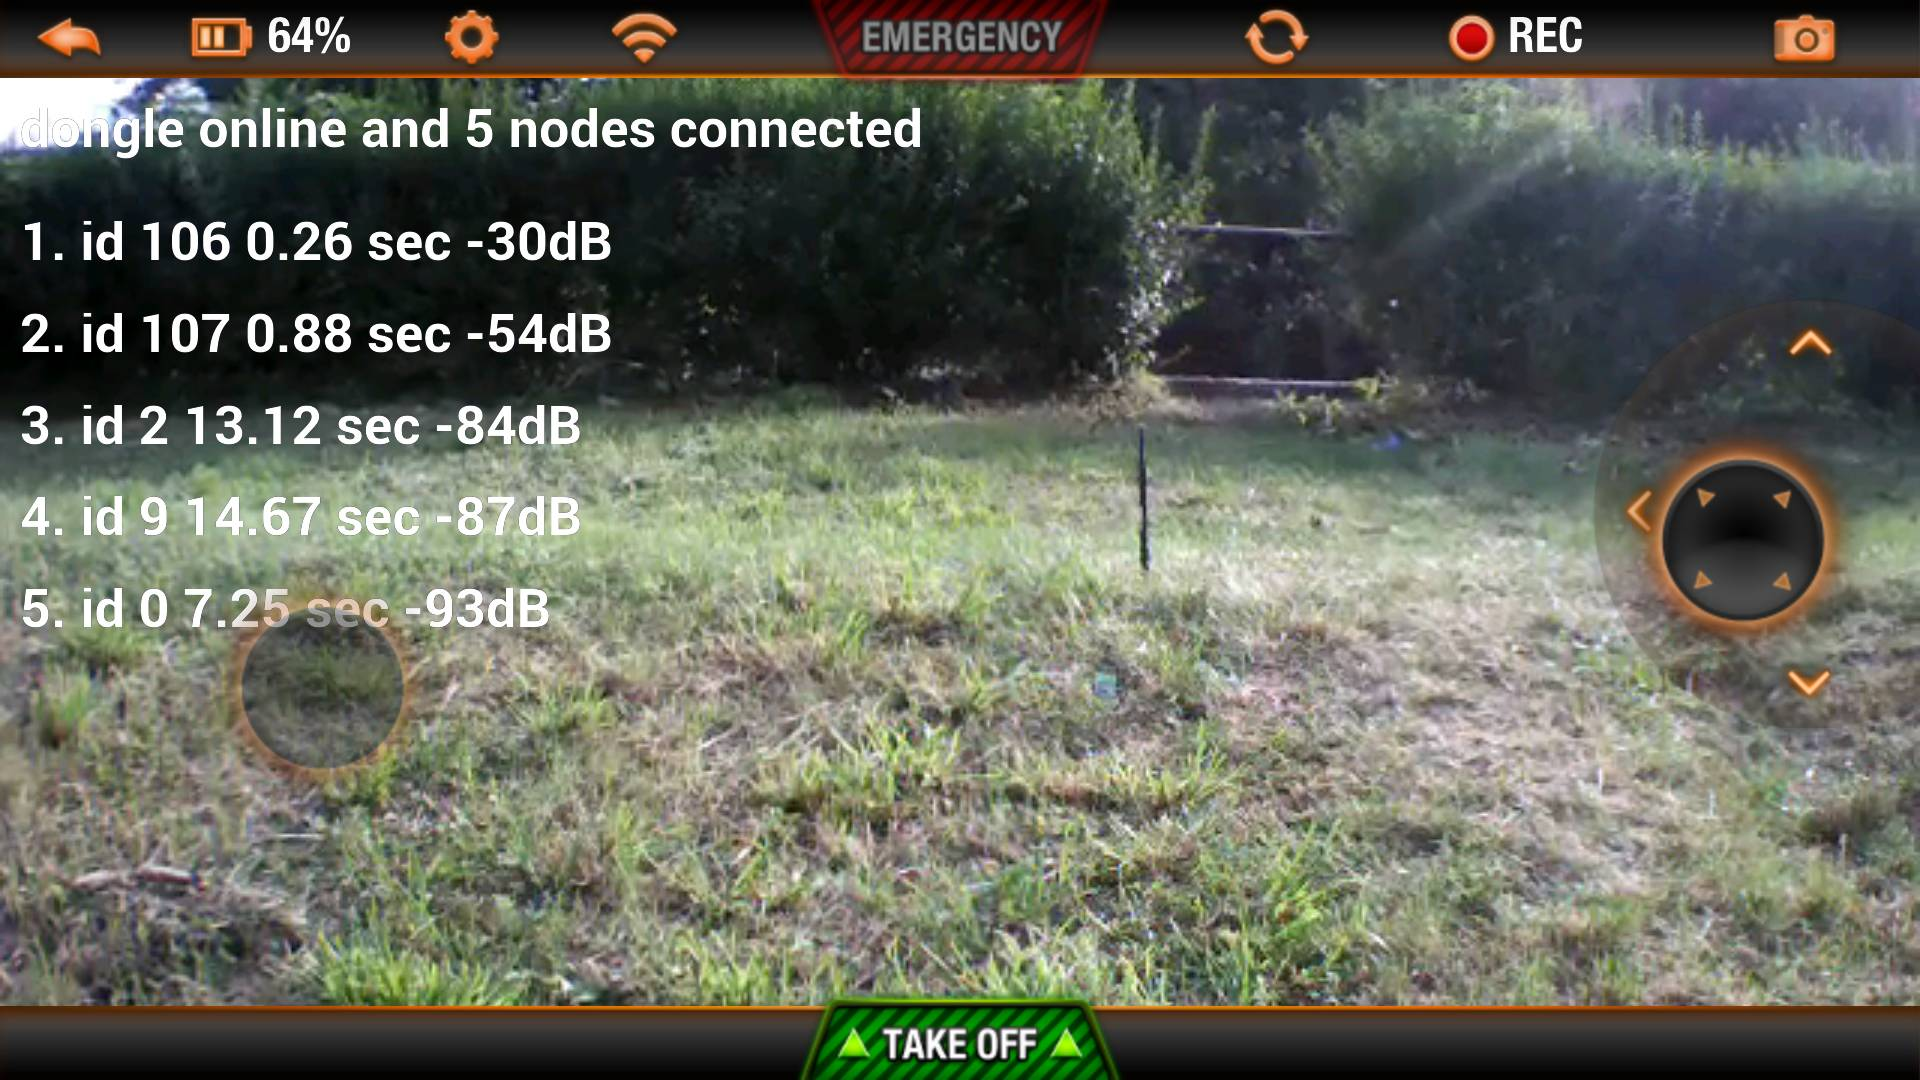
\includegraphics[width=0.9\textwidth]{img/parrot_test.png}
\end{center}
\caption{\small \itshape{Parrot discovering new nodes before takeoff}}
\end{figure}


\section{Results}

 
\subsection{Signal range}

\begin{figure}[ht]
  \label{fig:distance}
\begin{center}
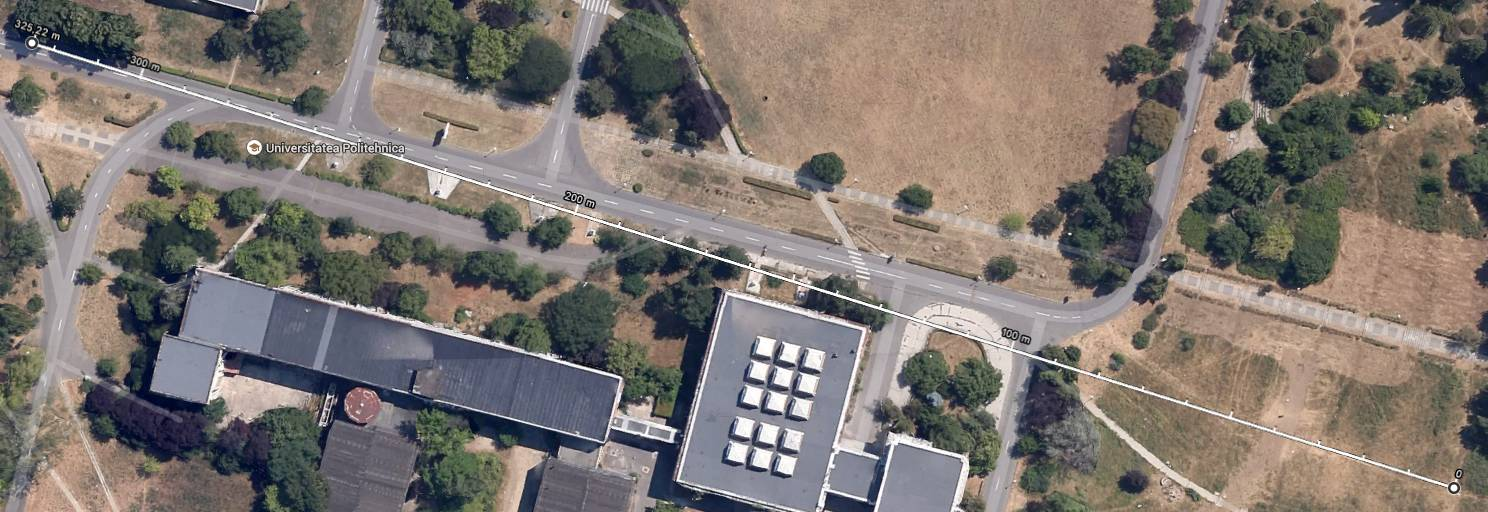
\includegraphics[width=0.9\textwidth]{img/distance.png}
\end{center}
\caption{\small \itshape{Measured signal distance}}
\end{figure}


The drone was able to find the nodes but, as depicted in figure~\ref{fig:discover}, the obstructed nodes had a much smaller communication range than the ones placed on the hill. The range test results proved that the drone could receive a signal at a maximum distance of 325 meters from the node with the 8 dBi external antenna located on the hill and a clear line of sight, highlighted in figure~\ref{fig:distance}. The other node on hill did manage to send data up to 100 meters. In the case of the obstructed nodes, even though they had a 3 dBi antenna, the distance did not exceeded the 45 meters mark. After this distance, the number of lost packets was to big to be able to properly communicate with the nodes, even though, occasionally, at 60 meters, some packets were received.


The top mounted antenna worked, but for a better signal quality, the antenna should always be positioned on the bottom of the drone. In this way, the antenna will have a clear path to send and receive signals and not be blocked by the drone body and its avionics. The problem with this particular drone model is that on its bottom there are sensors that help it determine the ground speed and ground distance. If we place the antenna on the bottom it would obstruct some of the sensors. A vertical antenna will increase wind resistance and make the drone too unstable.


\subsection{Drone stability}

Even though the antenna was mounted on top of the body, because it is a high gain antenna the signal received was very strong. 

The antenna, shown in figure~\ref{fig:antenna}, extended the signal range but also added weight. The dongle is mounted on the side of the drone due to the position of the USB connector. Because the dongle is not centered on the drone, a counterweight had to be glued on the opposite side on the outer shell to maintain the balance of the drone. 

The drone was relatively stable during tests, but a better stability and flight control could be obtained if the dongle were made smaller and a lighter antenna were used.


\begin{figure}[ht]
  \label{fig:antenna}
\begin{center}
\includegraphics[width=0.9\textwidth]{img/parrot_antenna.jpg}
\end{center}
\caption{\small \itshape{Top mounted antenna for better signal quality}}
\end{figure}



\subsection{Maximum height and maneuverability}

The total added weight is 75 grams. Even though it does not sound that much, it does have a substantial effect on the drone. The maximum height it can reach is 50 meters versus the 75 meters it can reach without the added weight. The maneuverability is also affected, the drone response not being as sharp as before, but it is still good.

\subsection{Problems}

The kernel module needed for the dongle does not recognize the dongle if it is plugged in the drone when its powering up. The fix is to power up the drone and then plug in the dongle, but this is more difficult than it might appear because every time this action is performed the hull must be repositioned.

\clearpage
